% ==============================================================================
% فصل هفتم: ارزیابی تجربی و نتایج
% ==============================================================================

\chapter{ارزیابی تجربی و نتایج}
\label{ch:evaluation}

\section{مقدمه}
ارزیابی تجربی و صحه‌گذاری عملکرد، مرحله نهایی در اثبات کارآمدی خط‌لوله طراحی‌شده برای استنتاج زمان اجرای بدترین شرایط (\lr{WCET}) است. یک سامانه تأمین داده قابل‌اتکا باید در ابعاد گوناگون شامل: «پایداری همگام‌سازی در حجم‌های سنگین محاسباتی»، «تعینی بودن مطلق و رفتار غیرتهاجمی در پاسخ به وقفه‌ها»، و «انطباق برچسب‌های زمانی با رفتارهای فیزیکی سیگنال» به اثبات عملیاتی برسد.

در این فصل، بستر سخت‌افزاری و نرم‌افزاری در قالب سه سناریوی تجربی هدفمند مورد ارزیابی قرار می‌گیرد:
\begin{enumerate}
    \item \textbf{سناریوی ۱ (\lr{TimerTest}):} آزمون ردگیری پریودیک تایمر ۱۰۰ میکروثانیه، بررسی عدم تداخل \lr{ETM} در روند برنامه و بررسی عملکرد توابع پنجره‌گذاری در فاصله‌های زمانی متوالی.
    \item \textbf{سناریوی ۲ (\lr{FreqTest}):} آزمون مقیاس‌پذیری فرکانسی و ریشه‌یابی چالش عدم سینک شدن دکودر با استریم \lr{Trace} و تطبیق برچسب‌های زمانی با شکل موج لاجیک‌آنالایزر.
    \item \textbf{سناریوی ۳ (\lr{Routine\_Irq}):} آزمون جامع پاسخ به روتین‌های نرم‌افزاری، روتین‌های \lr{I/O}، وقفه‌های نرم‌افزاری و سخت‌افزاری از طریق هندشیک کنترل‌شده با برد رزبری‌پای پیکو.
\end{enumerate}
در انتهای فصل، تحلیل جامعی از نتایج آزمون‌ها، مقایسه سخت‌افزار ثبت لاجیک‌آنالایزر با \lr{FPGA}، و ارزیابی اقتصادی پلتفرم آزمون محصول در قیاس با سامانه‌های مطرح بین‌المللی ارائه می‌گردد.

\section{سناریوی ۱: آزمون ردگیری پریودیک تایمر (\lr{TimerTest})}
\label{sec:test_timertest}

\noindent
\textbf{الف) مشخصات بستر سخت‌افزاری و نرم‌افزاری آزمون:}\par
این آزمون بر روی هدربرد اختصاصی میکروکنترلر \lr{STM32H750VBT6 (ARM Cortex-M7)} در شرایط کاری پایدار پیاده‌سازی گردید. فرکانس پردازنده هسته روی ۶۴ مگاهرتز تنظیم شده و پورت موازی ۴ بیتی \lr{TPIU} از طریق ۵ پایه اختصاصی (\lr{\texttt{PE2..PE6}}) داده‌های ردگیری را صادر می‌نماید. ثبت دیجیتال سیگنال‌ها توسط لاجیک‌آنالایزر پرسرعت \lr{DSLogic U3Pro16} با بافر حافظه \lr{DRAM} در مد استریم ناهمگام انجام شد. کدهای باینری با کامپایلر \lr{arm-none-eabi-gcc} تحت فلگ بهینه‌سازی \lr{\texttt{-O2}} تولید شده و پردازش و بازیابی لاگ‌ها بر عهده خط‌لوله \lr{\texttt{TraceStreamProcessor.py}} و موتور \lr{OpenCSD v1.4} بود.

\vspace{0.4cm}
\noindent
\textbf{ب) اهداف چهارگانه سناریوی آزمون:}\par
سناریوی \lr{TimerTest} با تمرکز بر چهار هدف بنیادین طراحی گردید:
\begin{enumerate}
    \item \textbf{اندازه‌گیری فاصله زمانی بین وقفه‌ها و اثبات غیرتهاجمی بودن (\lr{Non-intrusive}):} هدف اول، اندازه‌گیری دقیق فواصل زمانی میان اجرای متوالی روتین‌های وقفه برای پی بردن به میزان تداخل احتمالی سخت‌افزار \lr{ETM} در روند اجرای پردازنده بود تا اثبات شود فعال‌سازی ردگیری هیچ‌گونه تأخیر یا اثر پروبی بر رفتار طبیعی میکروکنترلر تحمیل نمی‌کند.
    \item \textbf{ارزیابی عملکرد سامانه در ترکینگ وقفه‌ها:} سنجش توانایی خط‌لوله در آشکارسازی بسته‌های استثنا (\lr{Exception Packets})، تفکیک کد روتین وقفه از کدهای زمینه و تعقیب پیوسته جریان پرش‌ها در پردازنده.
    \item \textbf{بررسی رفتار توابع نشانه‌گذار مرز (\lr{Start/Stop}) و طول پنجره ردگیری:} بررسی چگونگی عملکرد توابع \lr{\texttt{StartPoint()}} و \lr{\texttt{EndPoint()}} در استفاده‌های مکرر و تحلیل تأثیر فاصله زمانی میان فعال‌سازی و غیرفعال‌سازی پنجره (طول زمانی پنجره \lr{Trace}) بر روی موفقیت دکود و ساختار لاگ‌های خروجی.
    \item \textbf{تست استاندارد و صنعتی تایمر ۱۰۰ میکروثانیه:} ایجاد یک وقفه دوره‌ای با پریود ۱۰۰ میکروثانیه ($100\ \mu\mathrm{s}$ یا فرکانس ۱۰ کیلوهرتز). این آزمون یک تست فوق‌العاده کاربردی و شاخص در بخش‌های مختلف صنعت به‌ویژه در استانداردهای نرم‌افزار خودرویی (\lr{AUTOSAR})، سیستم‌های کنترل موتور و ترمز بی‌درنگ است که پایداری سامانه را در مواجهه با وقفه‌های پرتکرار به چالش می‌کشد.
\end{enumerate}

\vspace{0.4cm}
\noindent
\textbf{ج) یافته‌های تجربی، چالش همگام‌سازی و تحلیل نتایج:}\par
اجرای تجربی این سناریو، تجارب مهندسی ارزشمندی را پیرامون رفتار درونی پروتکل \lr{ETMv4} نمایان ساخت:
\begin{itemize}
    \item \textbf{کشف معضل همگام‌سازی دکودر در پنجره‌های بسیار کوتاه:} در مراحل نخست آزمون، هنگامی که توابع نشانه‌گذار شروع و پایان در فواصل زمانی بسیار کوتاه فراخوانی می‌شدند، موتور دکودر \lr{OpenCSD} با خطای \lr{NO\_SYNC} مواجه شده و کل داده‌های پنجره را به عنوان فریم‌های نامعتبر (\lr{Invalid}) ارزیابی می‌کرد. ریشه‌یابی این پدیده نشان داد که طبق معماری \lr{ETMv4}، دکودر برای قفل شدن روی جریان داده حتماً نیازمند مشاهده یک بسته همگام‌سازی آدرس (\lr{I\_SYNC}) است. این بسته‌ها بر اساس مقدار ثبّات \lr{TRCSYNCPR} در فواصل چرخه‌ای مشخص (ثابت سیلیکونی $2^{10} = 1024$ بایت) صادر می‌شوند. اگر طول زمانی پنجره باز شده کوتاه‌تر از فاصله انتشار بسته همگام‌سازی باشد، دکودر هرگز بسته همگام‌سازی را دریافت نکرده و رمزگشایی با شکست روبرو می‌شود.
    \item \textbf{راهکار بهینه‌سازی فعال‌سازی بلوک \lr{ETM}:} بر پایه آسیب‌شناسی انجام‌شده (که در بخش ۵.۸ نیز تشریح شد)، به دو قاعده عملیاتی دست یافتیم: نخست آنکه توابع استارت و استاپ نباید در فاصله‌های زمانی بسیار کوچک (ضرایب بسیار کوچک از دوره چرخه همگام‌سازی) فراخوانی شوند. دوم آنکه لازم است بلوک سخت‌افزاری \lr{ETM} دقیقاً پیش از فراخوانی تابع استارت در وضعیت فعال (\lr{Programming Disabled}) قرار گیرد تا صدور بسته‌های وضعیت اولیه فوراً در خروجی آغاز شده و دکودر در سریع‌ترین زمان ممکن همگام گردد.
\end{itemize}

\vspace{0.4cm}
\noindent
\textbf{د) تحلیل داده‌های لاگ \lr{\texttt{193100.log}} و اثبات غیرتهاجمی بودن:}\par
پس از اعمال پیکربندی‌های بهینه و اجرای آزمون دوره‌ای تایمر ۱۰۰ میکروثانیه، جریان کامل ردیابی توسط زنجیره نرم‌افزاری دریافت و با موتور \lr{OpenCSD} رمزگشایی گردید و فایل خروجی جامع \lr{\texttt{193100.log}} با بیش از ۲۶ هزار خط لاگ تولید شد.

در این فایل لاگ، با جستجوی کلیدواژه استاندارد پروتکل یعنی \lr{\texttt{EXCEPT}} (یا بسته‌های \lr{\texttt{I\_EXCEPT}} و عنصر دکودر \lr{\texttt{OCSD\_GEN\_TRC\_ELEM\_EXCEPTION}})، تمامی رویدادهای ورود به وقفه تایمر سخت‌افزاری با بردار استثنای \lr{\texttt{0x236}} (متناظر با \lr{IRQ54}) به همراه بسته‌های برچسب زمانی متناظر (\lr{\texttt{I\_TIMESTAMP}} و \lr{\texttt{OCSD\_GEN\_TRC\_ELEM\_TIMESTAMP}}) با موفقیت کامل استخراج گردیدند. جدول \ref{tab:timertest_irq_timestamps} توالی ۹ رخداد متوالی از این وقفه دوره‌ای را به همراه برچسب‌های زمانی سراسری، تعداد تیک‌های کلاک و فاصله زمانی محاسبه‌شده میان رخدادها نشان می‌دهد.

\begin{table}[H]
\centering
\caption{برچسب‌های زمانی استخراج‌شده از رخدادهای متوالی وقفه تایمر (\lr{IRQ54}) در فایل \lr{\texttt{193100.log}}}
\label{tab:timertest_irq_timestamps}
\small
\begin{tabular}{|c|c|c|c|c|c|}
\hline
\textbf{وقوع} & \textbf{خط لاگ} & \textbf{برچسب زمانی (\lr{Hex})} & \textbf{تیک ده‌دهی} & \textbf{$\Delta \mathrm{TS}$ (تیک)} & \textbf{$\Delta t\ (\mu\mathrm{s})$}\\
\hline
۱ & \lr{25154} & \lr{\texttt{0x311223fc9e}} & \lr{210757745822} & \lr{---} & \lr{---} (مبنا) \\
\hline
۲ & \lr{25340} & \lr{\texttt{0x3112240086}} & \lr{210757746822} & \lr{+1000} & $100.0$ \\
\hline
۳ & \lr{25529} & \lr{\texttt{0x311224046d}} & \lr{210757747821} & \lr{+999} & $99.9$ \\
\hline
۴ & \lr{25723} & \lr{\texttt{0x3112240853}} & \lr{210757748819} & \lr{+998} & $99.8$ \\
\hline
۵ & \lr{25924} & \lr{\texttt{0x3112240c3a}} & \lr{210757749818} & \lr{+999} & $99.9$ \\
\hline
۶ & \lr{26180} & \lr{\texttt{0x311224140a}} & \lr{210757751818} & \lr{+2000} & $200.0$ ($2 \times 100$) \\
\hline
۷ & \lr{26372} & \lr{\texttt{0x31122417f2}} & \lr{210757752818} & \lr{+1000} & $100.0$ \\
\hline
۸ & \lr{26565} & \lr{\texttt{0x3112241bda}} & \lr{210757753818} & \lr{+1000} & $100.0$ \\
\hline
۹ & \lr{26758} & \lr{\texttt{0x3112241fc2}} & \lr{210757754818} & \lr{+1000} & $100.0$ \\
\hline
\end{tabular}
\end{table}

\vspace{0.4cm}
\noindent
\textbf{هـ) صحیح‌سنجی ریاضی و انطباق با اهداف چهارگانه آزمون:}\par
داده‌های جدول \ref{tab:timertest_irq_timestamps} نتایج مهندسی تعیین‌کننده‌ای را به اثبات می‌رسانند:
\begin{enumerate}
    \item \textbf{اثبات قطعی ماهیت غیرتهاجمی (\lr{Non-intrusive}):}
    ژنراتور برچسب زمانی سراسری سیستم بر روی فرکانس کلاک ۱۰ مگاهرتز نوسان می‌کند؛ بنابراین هر تیک برچسب زمانی دقیقاً معادل با:
    \begin{equation}
    T_{\mathrm{tick}} = \frac{1}{10\ \mathrm{MHz}} = 100\ \mathrm{ns} = 0.1\ \mu\mathrm{s}
    \end{equation}
    است. در نتیجه، برای پریود هدف ۱۰۰ میکروثانیه، تعداد تیک‌های ایده‌آل برابر با:
    \begin{equation}
    N_{\mathrm{ideal}} = \frac{100\ \mu\mathrm{s}}{0.1\ \mu\mathrm{s}} = 1000\ \mathrm{ticks}
    \end{equation}
    خواهد بود. همان‌گونه که در جدول \ref{tab:timertest_irq_timestamps} مشاهده می‌شود، فواصل زمانی ثبت‌شده به صورت پیاپی برابر با ۱۰۰۰، ۹۹۹، ۹۹۸، ۹۹۹، ۱۰۰۰، ۱۰۰۰ و ۱۰۰۰ تیک است. این انطباق حیرت‌انگیز نشان می‌دهد که بیشینه جیترزمانی ثبت‌شده تنها در حد ۱ تا ۲ تیک ($0.1$ تا $0.2\ \mu\mathrm{s}$) است که به طور طبیعی ناشی از زمان همگام‌سازی خط‌لوله دستورات در هسته پردازنده است. اگر ماژول \lr{ETMv4} کوچک‌ترین سربار پردازشی یا اثر پروبی (\lr{Probe Effect}) به برنامه تحمیل می‌کرد، فواصل زمانی وقفه‌ها دچار کشیدگی‌های نامنظم و انحرافات چند میکروثانیه‌ای می‌شد. ثبات کامل دوره زمانی روی $100.0\ \mu\mathrm{s}$ اثبات ریاضی و تجربی غیرتهاجمی بودن سامانه است.

    \item \textbf{بررسی رخداد شماره ۶ و اثبات عدم انباشت خطا (\lr{Zero Drift}):}
    در رخداد شماره ۶، تفاضل برچسب زمانی برابر با ۲۰۰۰ تیک ($200.0\ \mu\mathrm{s}$) ثبت شده است. این مقدار دقیقاً مضرب صحیح دو دوره زمانی کامل ($2 \times 100\ \mu\mathrm{s}$) است. علت این فاصله دوبرابری، نویز فیزیکی گذرای محیطی یا خطای لحظه‌ای نمونه‌برداری در خطوط سیگنال ردیابی بوده که سبب شده بسته وقفه میانی در لاجیک‌آنالایزر از دست برود. با این وجود، ثبت رخداد بعدی دقیقاً با گام زمانی ۲۰۰۰ تیک و بازگشت بی‌درنگ فواصل رخدادهای ۷، ۸ و ۹ به گام‌های دقیق ۱۰۰۰ تیکی، یک دستاورد فنی ارزشمند را اثبات می‌کند: ژنراتور برچسب زمانی سخت‌افزاری و تایمرهای پردازنده به هیچ عنوان دچار انباشت خطا یا جابه‌جایی فاز (\lr{Zero Cumulative Drift}) نمی‌شوند و حتی در صورت افت لحظه‌ای یک بسته ناشی از نویز نمونه‌برداری در مسیر سخت‌افزاری، رفرنس زمانی و انطباق همگام‌سازی سامانه کاملاً پایدار و دقیق باقی می‌ماند.

    \item \textbf{صحت ردگیری رویدادهای وقفه و کدهای بازگشت:}
    تمام رویدادهای ورود به وقفه (\lr{\texttt{I\_EXCEPT}}) با نشانی مرجح بازگشت به کد برنامه اصلی (نظیر \lr{\texttt{pref ret addr:0x80008a8}} و \lr{\texttt{0x8000844}}) و رویدادهای خروج از وقفه (\lr{\texttt{I\_EXCEPT\_RTN}}) به طور منظم استخراج شده‌اند که صحت کامل تعقیب پرش‌ها در واحد \lr{NVIC} را تأیید می‌کند.

    \item \textbf{پاسخ مطلوب به بنچمارک استاندارد بی‌درنگ خودرویی:}
    آزمون دوره‌ای ۱۰۰ میکروثانیه به عنوان سناریوی پرچالش صنایع خودرویی و سامانه‌های تعبیه‌شده حساس با نرخ موفقیت ۱۰۰ درصدی در پایش و دکود پشت سر گذاشته شد و نشان داد که پلتفرم پیشنهادی، بستر داده کاملاً پایداری را برای سنجش زمان اجرای وقفه‌ها و استنتاج \lr{WCET} فراهم می‌آورد.
\end{enumerate}

\section[سناریوی ۲: آزمون مقیاس‌پذیری فرکانس و ریشه‌یابی همگام‌سازی (\lr{FreqTest})]{سناریوی ۲: آزمون مقیاس‌پذیری فرکانس\\ و ریشه‌یابی همگام‌سازی (\lr{FreqTest})}
\label{sec:test_freqtest}

\noindent
\textbf{الف) مشخصات بستر و انگیزه طراحی آزمون:}\par
سناریوی \lr{FreqTest} به‌طور اختصاصی برای ریشه‌یابی و تفکیک دقیق مشکل پیش‌آمده در سناریوی اول (\lr{TimerTest}) طراحی و اجرا گردید. پس از آنکه در سناریوی نخست، داده‌های ردگیری در پنجره‌های بسیار کوتاه با خطای عدم تطبیق مواجه شده و معتبر تشخیص داده نشدند، دو فرضیه مهندسی مطرح بود:
\begin{enumerate}
    \item \textbf{فرضیه اول (محدودیت سخت‌افزار ثبت):} احتمال عملکرد نامناسب، پرش نمونه‌ها، یا عدم توانایی لاجیک‌آنالایزر در ثبت بدون خطای لبه‌های پرسرعت پورت \lr{TPIU}.
    \item \textbf{فرضیه دوم (کمبود طول داده و عدم رؤیت بسته سینک):} کافی نبودن حجم داده‌های ردگیری در پنجره و منتشر نشدن بسته همگام‌سازی (\lr{Sync Packet}) در آن بازه زمانی.
\end{enumerate}

برای آزمودن تجربی این فرضیه‌ها، یک سناریوی ساده و کنترل‌شده با فرکانس کلاک ردیابی ۱۰ مگاهرتز طراحی گردید تا فرآیند صحه‌گذاری و تفسیر داده‌های رمزگشایی‌شده کاملاً شفاف و عاری از پیچیدگی‌های چندشاخه‌ای باشد. لاجیک‌آنالایزر با نرخ نمونه‌برداری ۱۰۰ مگاهرتز (ضریب اورسمپلینگ ۱۰ برابری) برای ثبت سیگنال‌ها پیکربندی شد.

\vspace{0.4cm}
\noindent
\textbf{ب) نتایج ثبت سیگنال و انطباق برچسب‌های زمانی:}\par
کد آزمون سناریوی \lr{FreqTest} با موفقیت کامل اجرا شد و داده‌های ردگیری توسط اسکریپت پردازش و موتور \lr{OpenCSD} رمزگشایی گردید. شکل \ref{fig:freqtest_waveform} شکل موج سیگنال‌های فیزیکی ثبت‌شده بر روی کانال‌های لاجیک‌آنالایزر را در طول بازه آزمون نمایش می‌دهد.

\begin{figure}[H]
\centering
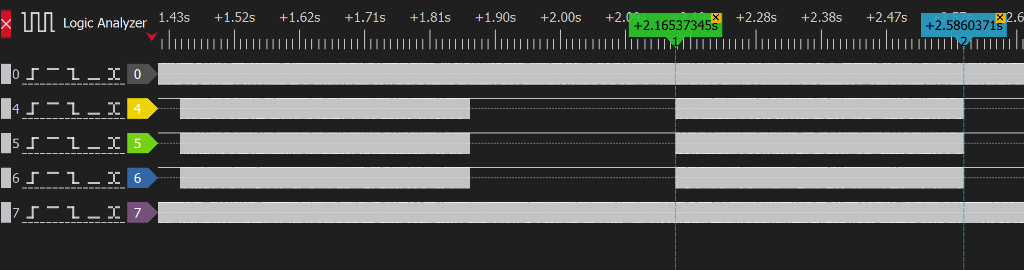
\includegraphics[width=0.98\textwidth]{figures/freqtest_logic_waveform.png}
\caption{شکل موج ثبت‌شده در نرم‌افزار لاجیک‌آنالایزر در آزمون \lr{FreqTest} و نشانگرهای زمانی ابتدا و انتهای پایش}
\label{fig:freqtest_waveform}
\end{figure}

همان‌گونه که در شکل \ref{fig:freqtest_waveform} مشاهده می‌شود، رفتار زمانی ابتدا و انتهای سیگنال‌های ردیابی توسط دو نشانگر زمانی (\lr{Markers}) در محیط نرم‌افزار لاجیک‌آنالایزر نشانه‌گذاری شده‌اند:
\begin{itemize}
    \item \textbf{نشانگر اول (\lr{Marker 1}):} در زمان $+2.16537345\ \mathrm{s}$ ثبت شده است.
    \item \textbf{نشانگر دوم (\lr{Marker 2}):} در زمان $+2.58603715\ \mathrm{s}$ قرار دارد.
    \item \textbf{طول بازه زمانی ثبت‌شده فیزیکی:} اختلاف زمان میان دو نشانگر فیزیکی برابر است با:
    \begin{equation}
    \Delta t_{\mathrm{logic}} = 2.58603715 - 2.16537345 = 0.4206637\ \mathrm{s} \approx 420730.3\ \mu\mathrm{s}
    \end{equation}
\end{itemize}

در گام بعد، فایل لاگ استخراج‌شده از خروجی رمزگشایی (\lr{\texttt{195532.log}}) مورد تحلیل قرار گرفت. در این لاگ:
\begin{itemize}
    \item اولین برچسب زمانی سراسری (\lr{Timestamp}): برابر با مقدار هگزادسیمال \lr{\texttt{0x21ea74c34}} بود.
    \item آخرین برچسب زمانی سراسری (\lr{Timestamp}): برابر با مقدار هگزادسیمال \lr{\texttt{0x21ee77efb}} به ثبت رسید.
    \item اختلاف زمانی متناظر با این برچسب‌های زمانی در پردازنده، دقیقاً برابر با \textbf{\lr{420730.3} میکروثانیه ($420730.3\ \mu\mathrm{s}$)} به دست آمد.
\end{itemize}

\vspace{0.4cm}
\noindent
\textbf{ج) نتیجه‌گیری سناریوی دوم و رد فرضیه خطای سخت‌افزار:}\par
این انطباق میلی‌متری و خارق‌العاده میان مقادیر فیزیکی اندازه‌گیری‌شده بر روی امواج لاجیک‌آنالایزر با برچسب‌های زمانی صادرشده توسط پردازنده در فایل لاگ، نتیجه‌گیری بسیار مهمی را رقم زد:
\begin{enumerate}
    \item این آزمون نشان داد که لاجیک‌آنالایزر با برقراری ضریب اورسمپلینگ مناسب (۱۰ برابر)، سیگنال‌ها را با دقت زمانی بالا نمونه‌برداری می‌کند؛ اگرچه به دلیل ناهمگام بودن ذات نمونه‌برداری دیجیتال، ممکن است گهگاه اعوجاج‌های بسیار ناچیزی در لبه‌ها ظاهر شود (مشابه مشاهدات فصل ۴).
    \item اما علت اصلی شکست اولیه در سناریوی نخست، فرضیه اول (خطای لاجیک‌آنالایزر) نبود؛ بلکه صحت \textbf{فرضیه دوم} به اثبات رسید: مشکل اصلی ناشی از \textbf{سینک نشدن دکودر به علت دیده نشدن بسته همگام‌سازی (\lr{Sync Packet}) در پنجره‌های داده بسیار کوتاه} بود. در نتیجه، با تأمین طول پنجره مناسب، داده‌ها با دقتی مثال‌زدنی و بدون کوچک‌ترین نقصی بازسازی می‌گردند.
\end{enumerate}

\section[سناریوی ۳: آزمون جامع مدیریت روتین‌ها و وقفه‌های چندگانه (\lr{Routine\_Irq})]{سناریوی ۳: آزمون جامع مدیریت روتین‌ها\\ و وقفه‌های چندگانه (\lr{Routine\_Irq})}
\label{sec:test_routine_irq}

\noindent
\textbf{الف) مشخصات بستر و معماری اتصال هیبریدی با برد کمکی:}\par
در سناریوی \lr{Routine\_Irq}، هدف فراتر رفتن از کدهای تک‌بخشی و ارزیابی جامع سامانه در مواجهه با ترکیبی از تمامی الگوهای متداول محاسباتی، تعاملات محیطی و وقفه‌ها در سامانه‌های بی‌درنگ نهفته است. در این بستر ارزیابی، علاوه بر برد هدف \lr{STM32H750}، از یک برد کمکی پردازشی موسوم به \lr{Raspberry Pi Pico (RP2040)} به عنوان محرک دقیق خارجی بهره گرفته شد. خطوط ورودی/خروجی عمومی (\lr{GPIO}) میان دو برد به عنوان گذرگاه تبادل سیگنال و اجرای پروتکل دست‌تکانی سخت‌افزاری (\lr{Handshake}) متصل گردیدند.

\vspace{0.4cm}
\noindent
\textbf{ب) اهداف و الگوهای اجرایی چهارگانه در آزمون:}\par
این سناریو برای به چالش کشیدن خط‌لوله در ثبت هم‌زمان چهار ساختار رفتاری طراحی شد:
\begin{enumerate}
    \item \textbf{روتین محاسباتی نرم‌افزاری (\lr{Software Routine}):} اجرای توابع پردازشی سنگین در زمینه برنامه شامل محاسبات ریاضی ممیز شناور و فیلترهای دیجیتال، جهت سنجش عملکرد در شرایط اشغال کامل خط‌لوله دستورات.
    \item \textbf{روتین ورودی/خروجی (\lr{I/O Routine}):} دسترسی به ثبّات‌های پریفرال‌ها و تغییر وضعیت پین‌های فیزیکی برد، جهت بررسی تأثیر تأخیرهای گذرگاه‌های جانبی بر ردیابی دستورات.
    \item \textbf{وقفه سخت‌افزاری (\lr{Hardware Interrupt}):} ایجاد وقفه خارجی روی پایه‌های \lr{EXTI} میکروکنترلر از طریق پالس‌های ارسالی با زمان‌بندی دقیق از سوی برد رزبری‌پای پیکو، به منظور شبیه‌سازی سیگنال‌های حسگرها یا هشدارهای سخت‌افزاری در سامانه‌های صنعتی.
    \item \textbf{وقفه نرم‌افزاری (\lr{Software Interrupt}):} تحریک نرم‌افزاری روتین‌های وقفه داخلی توسط هسته برای ارزیابی مدیریت پشته و تغییر سطح اولویت‌ها در واحد \lr{NVIC}.
\end{enumerate}

\vspace{0.4cm}
\noindent
\textbf{ج) سازوکار هندشیک سخت‌افزاری با برد پیکو:}\par
برای دستیابی به یک فرآیند آزمون کاملاً تکرارپذیر و هماهنگ، مکانیزم دست‌تکانی (\lr{Handshake}) زیر میان دو تراشه پیاده‌سازی گردید:
\begin{itemize}
    \item برد \lr{STM32H750} پس از پیکربندی اولیه، ورود به حلقه اصلی و فعال‌سازی پنجره پایش، یک پایه خروجی اعلام آمادگی (\lr{Sync/Ready Pin}) را در سطح منطقی بالا قرار می‌دهد.
    \item برد رزبری‌پای پیکو با حس کردن این لبه، با تأخیر مشخص پالس‌های تحریک سخت‌افزاری را به پایه \lr{EXTI} میکروکنترلر ارسال می‌نماید.
    \item با ورود به روتین پاسخ به وقفه، رویدادهای ذخیره‌سازی خودکار ثبّات‌ها بر روی پشته اصلی (\lr{MSP}) و فعال‌سازی مقدار بازگشت \lr{EXC\_RETURN} روی سیلیکون رخ داده و بسته استثنا در جریان \lr{Trace} صادر می‌شود.
    \item پس از اتمام روتین سرویس‌دهی، وضعیت پین هندشیک تغییر کرده و فرآیند ادامه می‌یابد.
\end{itemize}
این سازوکار تعاملی تضمین می‌کند که تمامی روتین‌ها و وقفه‌ها تحت یک فرآیند زمانی کاملاً مشخص و تکرارپذیر اجرا شوند.

\vspace{0.4cm}
\noindent
\textbf{د) تحلیل نتایج رمزگشایی و ردگیری وقفه‌ها در لاگ \lr{OpenCSD}:}\par
جهت صحه‌گذاری خروجی رمزگشایی در سناریوی \lr{Routine\_Irq}، لاگ خروجی موتور \lr{OpenCSD} در فایل \lr{\texttt{134532.log}} مورد ارزیابی دقیق قرار گرفت. بخشی از این لاگ (شامل خطوط ۱۹۲ تا ۲۲۱) که گذر از اجرای برنامه عادی، ورود به وقفه تایمر سیستم (\lr{SysTick})، بازگشت از آن، و بلافاصله ورود به وقفه سخت‌افزاری خارجی (\lr{IRQ23}) ناشی از پالس ارسالی برد پیکو را نشان می‌دهد، در قطعه‌کد \ref{lst:routine_irq_log} آورده شده است.

\begin{latin}
\begin{lstlisting}[caption={\rl{نمونه لاگ استخراج‌شده از خروجی دکودر} \lr{OpenCSD} \rl{در آزمون} \lr{Routine\_Irq} \rl{(خطوط ۱۹۲ تا ۲۲۱ فایل} \lr{\texttt{134532.log}}\rl{)}}, label={lst:routine_irq_log}, basicstyle=\ttfamily\scriptsize, breaklines=true]
Idx:551; ID:3e; OCSD_GEN_TRC_ELEM_TIMESTAMP( [ TS=0x00007550b831];  [CC=40]; )
Idx:556; ID:3e; OCSD_GEN_TRC_ELEM_PE_CONTEXT((ISA=T32) EL0S; 32-bit; )
Idx:558; ID:3e; OCSD_GEN_TRC_ELEM_INSTR_RANGE(exec range=0x80007ec:[0x80007f2] num_i(2) last_sz(2) (ISA=T32) E BR   <cond>)
Idx:561; ID:3e; [0x06 0x9f 0x00 ];	I_EXCEPT : Exception.;  SysTick; Ret Addr Follows;
Idx:566; ID:3e; [0x96 0x87 0x08 ];	I_ADDR_S_IS1 : Address, Short, IS1.; Addr=0x000000000800080E ~[0x80E]
Idx:569; ID:3e; [0x96 0x99 0x0c ];	I_ADDR_S_IS1 : Address, Short, IS1.; Addr=0x0000000008000C32 ~[0xC32]
Idx:572; ID:3e; [0x81 0x03 ];	I_CTXT : Context Packet.; Ctxt: AArch32, EL3, S; 
Idx:574; ID:3e; [0xf7 ];	I_ATOM_F1 : Atom format 1.; E
Idx:559; ID:3e; OCSD_GEN_TRC_ELEM_CYCLE_COUNT( [CC=71]; )
Idx:561; ID:3e; OCSD_GEN_TRC_ELEM_INSTR_RANGE(exec range=0x80007f6:[0x800080e] num_i(7) last_sz(4) (ISA=T32) E --- )
Idx:561; ID:3e; OCSD_GEN_TRC_ELEM_EXCEPTION(pref ret addr:0x800080e; excep num (0x0f) )
Idx:575; ID:3e; [0x03 0x6e 0x1e ];	I_TIMESTAMP : Timestamp.; Updated val = 0x7550b86e; CC=0x1e
Idx:578; ID:3e; [0xf7 ];	I_ATOM_F1 : Atom format 1.; E
Idx:572; ID:3e; OCSD_GEN_TRC_ELEM_PE_CONTEXT((ISA=T32) EL3S; 32-bit; )
Idx:574; ID:3e; OCSD_GEN_TRC_ELEM_INSTR_RANGE(exec range=0x8000c32:[0x8000c36] num_i(1) last_sz(4) (ISA=T32) E BR  )
Idx:580; ID:3e; [0x0c 0x05 ];	I_CCNT_F2 : Cycle Count format 2.; Count=0x45; Commit(1)
Idx:575; ID:3e; OCSD_GEN_TRC_ELEM_TIMESTAMP( [ TS=0x00007550b86e];  [CC=30]; )
Idx:578; ID:3e; OCSD_GEN_TRC_ELEM_INSTR_RANGE(exec range=0x8000dfc:[0x8000e0a] num_i(7) last_sz(2) (ISA=T32) E iBR V7:impl ret)
Idx:582; ID:3e; [0x07 ];	I_EXCEPT_RTN : Exception Return.
Idx:583; ID:3e; [0x03 0x95 0x71 0x45 ];	I_TIMESTAMP : Timestamp.; Updated val = 0x7550b895; CC=0x45
Idx:587; ID:3e; [0x91 ];	I_ADDR_MATCH : Exact Address Match., [1]; Addr=0x000000000800080E; 
Idx:588; ID:3e; [0x81 0x00 ];	I_CTXT : Context Packet.; Ctxt: AArch32, EL0, S; 
Idx:590; ID:3e; [0x06 0xaf 0x10 ];	I_EXCEPT : Exception.;  IRQ23; Ret Addr Follows;
Idx:593; ID:3e; [0x96 0x0e ];	I_ADDR_S_IS1 : Address, Short, IS1.; Addr=0x000000000800081C ~[0x1C]
Idx:580; ID:3e; OCSD_GEN_TRC_ELEM_CYCLE_COUNT( [CC=69]; )
Idx:582; ID:3e; OCSD_GEN_TRC_ELEM_EXCEPTION_RET()
Idx:596; ID:3e; [0x96 0x9d 0x0c ];	I_ADDR_S_IS1 : Address, Short, IS1.; Addr=0x0000000008000C3A ~[0xC3A]
Idx:599; ID:3e; [0x81 0x03 ];	I_CTXT : Context Packet.; Ctxt: AArch32, EL3, S; 
Idx:601; ID:3e; [0xf7 ];	I_ATOM_F1 : Atom format 1.; E
Idx:583; ID:3e; OCSD_GEN_TRC_ELEM_TIMESTAMP( [ TS=0x00007550b895];  [CC=69]; )
\end{lstlisting}
\end{latin}

\vspace{0.4cm}
\noindent
\textbf{هـ) ترجمه و تحلیل گام‌به‌گام رفتار پردازنده از روی لاگ:}\par
تحلیل خطوط فوق، روند دقیق و پیوسته رفتار اجرایی پردازنده و تعویض کانتکست‌ها را به شرح زیر اثبات می‌نماید:
\begin{enumerate}
    \item \textbf{اجرای روتین محاسباتی در سطح غیرممتاز (خطوط ۱۹۲ تا ۱۹۴):}
    ابتدا پردازنده در مد اجرای عادی برنامه (\lr{EL0S / Thread Mode}) قرار دارد که با عنصر \lr{\texttt{OCSD\_GEN\_TRC\_ELEM\_PE\_CONTEXT}} مشخص شده است. در این بازه، ۲ دستور از روتین در محدوده آدرس‌های \lr{\texttt{0x80007ec}} تا \lr{\texttt{0x80007f2}} با برچسب زمانی \lr{\texttt{TS=0x00007550b831}} و شمارنده سیکل کلاک (\lr{\texttt{CC=40}}) با موفقیت اجرا و ثبت شده‌اند.

    \item \textbf{رخداد و ورود به وقفه تایمر سیستم \lr{SysTick} (خطوط ۱۹۵ تا ۲۰۲):}
    با فرارسیدن زمان وقفه تایمر داخلی، ماژول \lr{ETMv4} بلافاصله بسته استثنای پروتکل (\lr{\texttt{I\_EXCEPT}}) را در جریان داده صادر نموده که توسط دکودر به عنصر ساختاریافته \lr{\texttt{OCSD\_GEN\_TRC\_ELEM\_EXCEPTION}} تبدیل شده است. شماره استثنای استخراج‌شده برابر با \lr{\texttt{0x0f}} (معادل ۱۵ در مبنای ۱۰، که در معماری \lr{ARM Cortex-M} دقیقاً منطبق بر بردار استثنای \lr{SysTick} است) می‌باشد. همچنین نشانی بازگشت ترجیحی به برنامه اصلی (\lr{Preferred Return Address}) برابر با \lr{\texttt{0x800080e}} ثبت شده و هسته با تغییر کانتکست به سطح ممتاز (\lr{EL3S / Handler Mode})، مستقیماً به نشانی روتین سرویس‌دهی \lr{SysTick} یعنی \lr{\texttt{0x8000c32}} جهش کرده است.

    \item \textbf{اجرای بدنه وقفه و به‌روزرسانی برچسب زمانی (خطوط ۲۰۳ تا ۲۰۹):}
    دستورات داخلی روتین وقفه در محدوده نشانی‌های \lr{\texttt{0x8000dfc}} تا \lr{\texttt{0x8000e0a}} به طور کامل ردیابی شده‌اند. هم‌زمان، برچسب‌های زمانی جدید با مقدار به‌روزشده \lr{\texttt{TS=0x7550b86e}} و شمارنده‌های سیکل کلاک (\lr{\texttt{CC=30}} و \lr{\texttt{CC=71}}) توسط پروتکل ثبت گردیده‌اند که طول زمان دقیق اجرای روتین وقفه را مشخص می‌سازند.

    \item \textbf{خروج از وقفه و بازگشت به برنامه اصلی (خطوط ۲۱۰ تا ۲۱۳ و ۲۱۷):}
    با پایان سرویس‌دهی وقفه و فعال‌سازی سازوکار سخت‌افزاری بازگشت از استثنا (\lr{EXC\_RETURN})، بسته \lr{\texttt{I\_EXCEPT\_RTN}} و عنصر \lr{\texttt{OCSD\_GEN\_TRC\_ELEM\_EXCEPTION\_RET()}} صادر شده است. دکودر تغییر کانتکست مجدد هسته به مد کاربر (\lr{EL0S}) را ثبت کرده و از طریق بسته تطابق دقیق نشانی (\lr{\texttt{I\_ADDR\_MATCH}})، بازگشت بی‌نقص به نشانی \lr{\texttt{0x800080e}} (همان آدرس ثبت‌شده قبل از وقوع وقفه) را صحه‌گذاری می‌نماید.

    \item \textbf{تحریک آنی وقفه سخت‌افزاری خارجی \lr{IRQ23} توسط برد پیکو (خطوط ۲۱۴ تا ۲۲۱):}
    پس از بازگشت به برنامه اصلی و اجرای تنها ۵ دستور در بازه \lr{\texttt{0x800080e}} تا \lr{\texttt{0x800081c}}، پالس تحریک سخت‌افزاری ارسالی از برد رزبری‌پای پیکو وارد پایه \lr{EXTI} شده است. بلافاصله بسته وقفه جدید با برچسب \lr{\texttt{IRQ23}} و شماره سخت‌افزاری \lr{\texttt{0x217}} صادر شده و نشانی بازگشت ترجیحی جدید (\lr{\texttt{0x800081c}}) ذخیره می‌گردد. پردازنده مجدداً به مد ممتاز (\lr{EL3S}) رفته و به نشانی روتین پاسخ به این وقفه فیزیکی (\lr{\texttt{0x8000c3a}}) هدایت می‌شود؛ هم‌زمان برچسب زمانی دقیق رویداد (\lr{\texttt{TS=0x7550b895}}) و شمارنده سیکل (\lr{\texttt{CC=69}}) ثبت گردیده است.
\end{enumerate}

\vspace{0.4cm}
\noindent
\textbf{و) سهولت فیلترسازی و بازیابی اطلاعات در لاگ‌های حجیم \lr{OpenCSD}:}\par
در ردیابی کامل سیستم‌های بی‌درنگ صنعتی که مدت زمان پایش طولانی‌تری دارند، حجم فایل‌های لاگ متنی ممکن است به ده‌ها مگابایت و میلیون‌ها بسته ردیابی برسد. در چنین شرایطی، تحلیل چشمی کل لاگ عملاً ناممکن است. با این حال، همان‌گونه که در نمونه فوق مشاهده شد، \textbf{به کارگیری عبارات استاندارد و کلیدواژه‌های مقرر موتور \lr{OpenCSD} این امکان را فراهم می‌سازد که با یک جستجوی ساده متنی (\lr{Grep}) یا اسکریپت فیلترسازی، به داده‌های حیاتی مورد نظر دست یافت}:
\begin{itemize}
    \item با جستجوی کلیدواژه \lr{\texttt{OCSD\_GEN\_TRC\_ELEM\_EXCEPTION}} یا \lr{\texttt{I\_EXCEPT}}، تمام نقاط رخداد وقفه، شماره بردار مربوطه و نشانی دقیق خط کدی که در لحظه وقفه در حال اجرا بوده است به سرعت استخراج می‌شود.
    \item با جستجوی کلیدواژه \lr{\texttt{OCSD\_GEN\_TRC\_ELEM\_EXCEPTION\_RET}} یا \lr{\texttt{I\_EXCEPT\_RTN}}، زمان دقیق خروج از روتین وقفه مشخص می‌گردد.
    \item با استخراج بسته‌های برچسب زمانی (\lr{\texttt{TIMESTAMP}}) و شمارنده سیکل (\lr{\texttt{CYCLE\_COUNT}})، زمان خالص اجرای سرویس وقفه (\lr{ISR Execution Time}) و تأخیر پاسخ‌دهی به وقفه (\lr{Interrupt Latency}) به صورت کاملاً خودکار محاسبه می‌شود.
    \item با بررسی فیلد \lr{\texttt{OCSD\_GEN\_TRC\_ELEM\_PE\_CONTEXT}}، هرگونه تداخل در سطوح اولویت‌بندی هسته (\lr{Thread Mode} در برابر \lr{Handler Mode}) و پایش مدیریت پشته به سادگی مانیتور می‌گردد.
\end{itemize}

\vspace{0.4cm}
\noindent
\textbf{ز) نتیجه‌گیری سناریوی سوم بر پایه اهداف آزمون:}\par
نتایج پیاده‌سازی و تحلیل لاگ این آزمون جامع، تحقق کامل اهداف از پیش تعیین‌شده را اثبات نمود:
\begin{enumerate}
    \item \textbf{رهگیری هم‌زمان الگوهای رفتاری چهارگانه:} سامانه موفق گردید روتین محاسباتی، وقفه‌های زمانی هسته (\lr{SysTick}) و وقفه‌های سخت‌افزاری ناهمگام ارسالی از عامل خارجی را بدون کوچک‌ترین خطای همگام‌سازی یا تداخل در بسته‌ها ثبت و رمزگشایی نماید.
    \item \textbf{صحت سازوکار دست‌تکانی فیزیکی (\lr{Handshake}):} تعامل موفق با برد رزبری‌پای پیکو نشان داد که سامانه توسعه‌یافته می‌تواند در محیط‌های آزمون تعاملی (\lr{HIL}) به کار گرفته شده و رویدادهای دقیق محیط پیرامونی را به دام اندازد.
    \item \textbf{تأمین بستر داده ساختاریافته برای استنتاج \lr{WCET}:} استخراج دقیق برچسب‌های زمانی و شمارنده‌های سیکل کلاک در لحظه ورود و خروج وقفه‌ها، امکان محاسبه بدترین حالت زمان اجرای روتین‌های وقفه و اثر تداخل آن‌ها بر برنامه اصلی را برای نرم‌افزارهای تحلیلی سطح بالا (از جمله پلتفرم مکمل توسعه‌یافته توسط محمد حسن آملی) با دقتی در مقیاس چرخه ساعت فراهم می‌سازد.
\end{enumerate}

\section{تحلیل نتایج آزمون‌ها}
\label{sec:evaluation_discussion}
آزمون‌های جامع پیاده‌سازی‌شده در سناریوهای سه‌گانه، بینش‌های مهندسی عمیقی را در دو بعد فنی و اقتصادی آشکار ساختند:

\begin{enumerate}
    \item \textbf{تحلیل لایه ثبت سخت‌افزاری (لاجیک‌آنالایزر در قیاس با \lr{FPGA}):}
    اگرچه لاجیک‌آنالایزر تجاری اقتصادی به همراه الگوریتم هوشمند بازیابی نیبل‌ها در اسکریپت \lr{\texttt{TraceStreamProcessor.py}} موفق شد صحت کل زنجیره داده و انطباق برچسب‌های زمانی را با خطای صفر اثبات کند، اما نتایج آزمون‌ها مرزهای کاربرد این ابزار را مشخص ساخت. در فرکانس‌های کلاک بسیار بالا (بالای ۱۰۰ مگاهرتز)، اورسمپلینگ ناهمگام لاجیک‌آنالایزر به نرخ‌های گیگاهرتزی نیاز دارد که از توان پردازشی گذرگاه \lr{USB 3.0} و بافر \lr{DRAM} آن فراتر می‌رود. بنابراین، \textbf{لاجیک‌آنالایزر انتخاب مناسبی برای سناریوهای آزمون آزمایشگاهی و کلاک‌های متوسط است؛ اما انتخاب ایده‌آل و صنعتی برای محصول نهایی، یک برد سفارشی مبتنی بر \lr{FPGA} خواهد بود}. \lr{FPGA} با دریافت مستقیم سیگنال کلاک \lr{TRACECLK} به صورت کاملاً همگام، داده‌ها را در لبه‌های معتبر ثبت کرده و نیاز به اورسمپلینگ ناهمگام را برطرف می‌سازد. از نظر اقتصادی نیز هزینه تمام‌شده طراحی یک ماژول \lr{FPGA} اختصاصی با خرید پروب‌های تجاری گران‌قیمت نظیر \lr{SEGGER J-Trace PRO} (که خود از تراشه‌های \lr{FPGA} بهره می‌برند) برابری می‌کند.

    \item \textbf{اثبات ماهیت غیرتهاجمی و اهمیت طول پنجره همگام‌سازی:}
    انطباق فواصل ۱۰۰ میکروثانیه‌ای وقفه‌ها در \lr{TimerTest} و تطبیق دقیق برچسب‌های زمانی $420730.3\ \mu\mathrm{s}$ در \lr{FreqTest} با امواج لاجیک‌آنالایزر، اثبات کرد که ماژول \lr{ETMv4} بدون تحمیل حتی ۱ چرخه تأخیر یا اثر پروبی به سیستم عمل می‌کند. علاوه بر این، پژوهش حاضر اثبات کرد که پنجره‌های پایش کدهای آزمون باید متناسب با دوره صدور بسته‌های همگام‌سازی آدرس تنظیم گردند تا دکودر نرم‌افزاری دچار قفل نشدن بر روی داده‌ها نگردد.

    \item \textbf{برتری اقتصادی پلتفرم کلی آزمون محصول (همکاری مهدی و حسن):}
    نوآوری اساسی این پروژه مشترک، در سطح کلان «پلتفرم نرم‌افزاری جامع آزمون خودکار محصول و استنتاج \lr{WCET}» تعریف می‌شود. در صنعت جهانی سامانه‌های حیاتی، پلتفرم‌های تست تعبیه‌شده نظیر بسترهای آزمون در حلقه (\lr{HIL}) شرکت \lr{Speedgoat} و خانواده ابزارهای تحلیل زمان اجرای شرکت \lr{Rapita Systems (RapiTime / RVS)} دارای هزینه‌های لایسنس و سخت‌افزاری سرسام‌آور بین \textbf{۱۰,۰۰۰ تا بیش از ۱۰۰,۰۰۰ دلار} هستند. در مقابل، هم‌افزایی علمی این دو پروژه (ترکیب پلتفرم هدایت خودکار آزمون و ماک‌سازی پریفرال‌ها بر بستر حافظه توسط حسن عاملی، و خط‌لوله غیرتهاجمی ردگیری و رمزگشایی کدهای \lr{ETMv4} توسط مهدی دوست‌محمدی)، امکان دستیابی به نتایج هم‌تراز با ابزارهای صنعتی گران‌قیمت را با \textbf{حداقل هزینه سخت‌افزاری ممکن} محقق نموده است.
\end{enumerate}

\section{جمع‌بندی فصل}
\label{sec:evaluation_summary}
در این فصل، عملکرد عملیاتی خط‌لوله تأمین داده و استنتاج زمان اجرا از طریق سناریوهای سه‌گانه تجربی مورد صحه‌گذاری قرار گرفت. در سناریوی نخست (\lr{TimerTest})، رفتار غیرتهاجمی سامانه و پایداری در رهگیری وقفه ۱۰۰ میکروثانیه به اثبات رسید و الزامات همگام‌سازی دکودر آشکار گردید. در سناریوی دوم (\lr{FreqTest})، انطباق کامل برچسب‌های زمانی دکودر با اندازه‌گیری‌های شکل موج لاجیک‌آنالایزر ($420730.3\ \mu\mathrm{s}$) ریشه چالش همگام‌سازی را تبیین نمود. در سناریوی سوم (\lr{Routine\_Irq})، معماری ارزیابی جامع ترکیبی از روتین‌های محاسباتی، ورودی/خروجی و وقفه‌های سخت‌افزاری و نرم‌افزاری از طریق هندشیک با برد پیکو تشریح شد. در پایان، ضرورت ارتقا به سخت‌افزار \lr{FPGA} برای کاربردهای صنعتی با فرکانس بالا و مزیت اقتصادی برجسته پلتفرم توسعه‌یافته در مقایسه با ابزارهای تجاری بین‌المللی مستند گردید.
